\documentclass{article}

\usepackage{hyperref}
\usepackage{amsmath}
\usepackage{subcaption}
\usepackage{graphicx}

% Page layout
\hoffset -0in
\voffset -1in
\oddsidemargin 0in
\textheight 10in
\textwidth 6.3in

\setlength{\parindent}{0pt}
\setlength{\intextsep}{10pt}
%\pagestyle{empty}

\graphicspath{{figures/}}

\begin{document}
	\section*{COMPUTATIONAL METHODS IN MECHANICS: Task 2}
	Vesa-Ville Hurskainen, 30 Jan 2018
	
	\section*{Introduction}
	This is a report on the second assignment of the course \textit{Computational Methods in Mechanics}, concerning the numerical solution of the dynamic response of a mass-spring-damper system using MATLAB. Five tasks were given, which are as follows:
	
	\begin{enumerate}
		\setlength\itemsep{0pt}
		\item To use GitHub.
		\item To create a MATLAB code that solves a mass-spring-damper system.
		\item To compare the exact solution for free and damped vibrations using different ODE solvers.
		\item To reduce the error in position by adjusting solver settings.
		\item To analyze forced and slightly damped vibrations with harmonic force, and investigate what happens when the force frequency passes the damped natural frequency and how the rate of change of the force frequency affects the solution.
	\end{enumerate}
	
	\section*{Methods}
	Denoting displacement with $x$ and external force with $F$, the equation of motion for the mass-spring-damper system can be written as
	\begin{equation}
		m \ddot{x} + c \dot{x} + k x  = F
	\end{equation}
	where $m$ is mass, $c$ is viscous damping coefficient and $k$ is spring coefficient. Here, the force was given as
	\begin{equation}
		F(t) = A \sin(\omega(t) t)
	\end{equation}
	where $A$ is harmonic force amplitude and $\omega$ is frequency. The analytically derived response function of the system, presuming that $F=0$ and system is underdamped (damping ratio $<$ 1), can be written as
	\begin{equation}
		x(t) = e^{-\zeta \omega_n t} \left(\frac{\dot{x}_0 + \zeta \omega_n x_0}{\omega_d} \sin(\omega_d t) + x_0 \cos(\omega_d t)\right)
	\end{equation}
	where damping ratio $\zeta = \frac{c}{2 \sqrt{km}}$, undamped natural frequency $\omega_n = \sqrt{\frac{k}{m}}$ and damped natural frequency $\omega_d = \omega_n \sqrt{1-\zeta^2}$. The initial values for displacement and velocity are $x_0$ and $\dot{x}_0$, respectively.
	
	\section*{Results}
	poop

	\section*{Analysis}
	The completion of the second and third tasks can be verified from Figure~\ref*{fig:response}. The numerical and analytical solutions coincide with a fair degree of accuracy in all cases, but consistently the best results were gained using the solver ode45 and the worst using ode23. The completion of task four can be verified from Table~\ref{tab:error_comparison}, which shows a significant decrease in error with tighter tolerances.\\
	
	The fifth task required ... ~\ref{fig:forced_response} \\
	
	The first task was completed by uploading the employed scripts and the source files of this report into a \href{https://github.com/VesaVilleHurskainen/cmim2018}{GitHub repository} using the MATLAB-integrated functions. Therefore, all tasks are judged to be complete.
	
	\clearpage
		\begin{figure}[h]
		\centering
		\begin{subfigure}[t]{0.45\textwidth}
			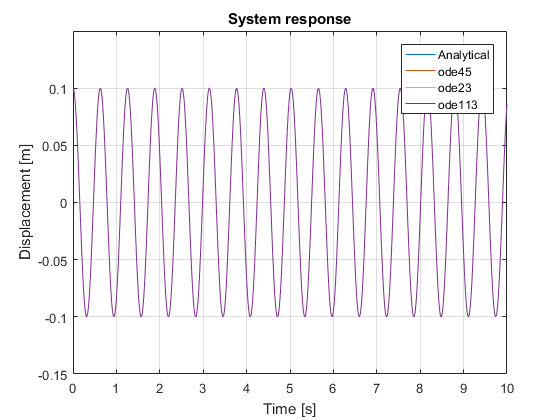
\includegraphics[width=\textwidth]{response_comparison_undamped.png}
			\caption{Response, $\zeta = 0$.}
		\end{subfigure}
		~
		\begin{subfigure}[t]{0.45\textwidth}
			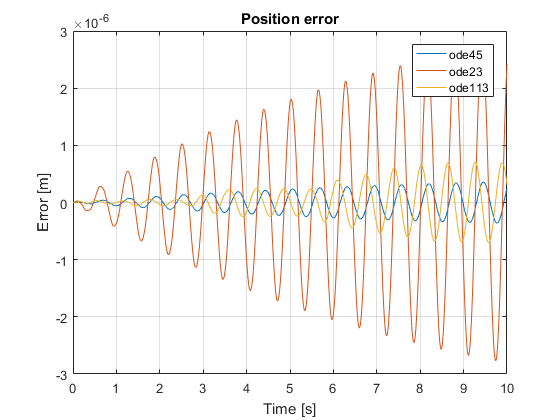
\includegraphics[width=\textwidth]{error_comparison_damped.png}
			\caption{Position error, $\zeta = 0$.}
		\end{subfigure}
		
		\begin{subfigure}[t]{0.45\textwidth}
			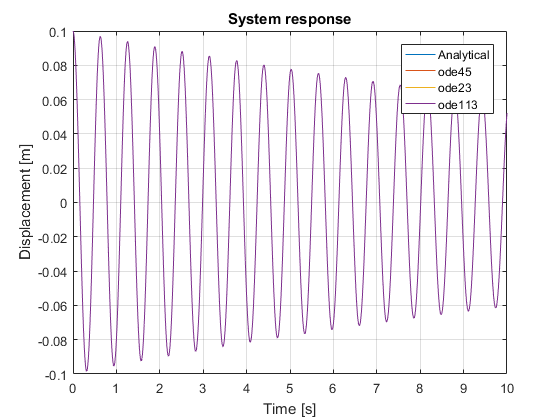
\includegraphics[width=\textwidth]{response_comparison_damped.png}
			\caption{Response, $\zeta = 0.1$.}
		\end{subfigure}
		~
		\begin{subfigure}[t]{0.45\textwidth}
			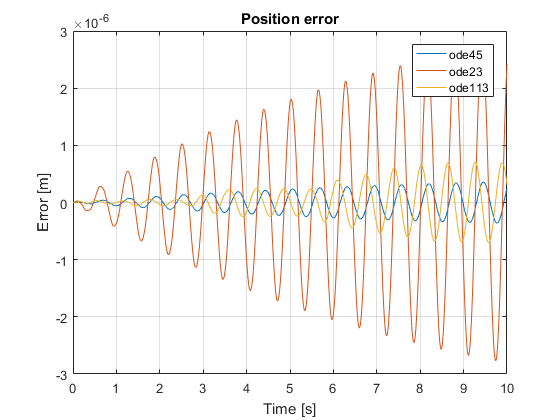
\includegraphics[width=\textwidth]{error_comparison_damped.png}
			\caption{Position error, $\zeta = 0.1$.}
		\end{subfigure}
		\caption{System response comparison, undamped and damped cases. Default solver options.}
		\label{fig:response}
	\end{figure}
	
	\begin{table}[h]
		\def\arraystretch{1.2}
		\begin{subtable}[t]{0.45\textwidth}
			\centering
			\begin{tabular}{|l|l|l|}
				\hline
				Solver & $\zeta = 0$ & $\zeta = 0.1$\\
				\hline
				ode45  & 1016 & 621.4 \\
				ode23  & 5042 & 3100 \\
				ode113 & 1482 & 953.4 \\
				\hline
			\end{tabular}
			\caption{Default options.}
		\end{subtable}
		~
		\begin{subtable}[t]{0.45\textwidth}
			\centering
			\begin{tabular}{|l|l|l|}
				\hline
				Solver & $\zeta = 0$ & $\zeta = 0.1$\\
				\hline
				ode45  & 0.5887 & 0.3609 \\
				ode23  & 4.506 s & 2.770 \\
				ode113 & 0.6283 & 0.7028 \\
				\hline
			\end{tabular}
			\caption{AbsTol = 1e-9, RelTol = 1e-3 .}
		\end{subtable}
		\caption{Comparison of maximum errors [$10^{-6}$ m].}
		\label{tab:error_comparison}
	\end{table}
	
	\begin{figure}[h]
		\centering
		\begin{subfigure}[t]{0.45\textwidth}
			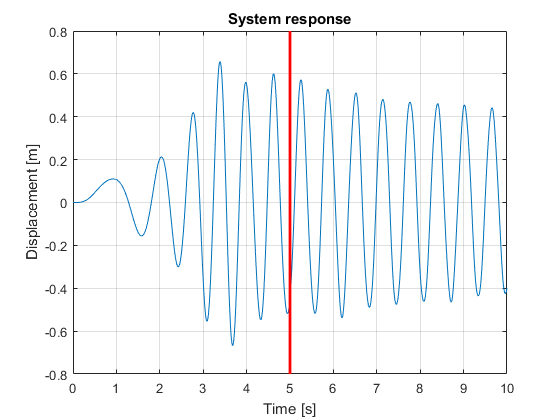
\includegraphics[width=\textwidth]{forced_response_slow.png}
			\caption{Response, $\omega = 2 t$ .}
		\end{subfigure}
		~
		\begin{subfigure}[t]{0.45\textwidth}
			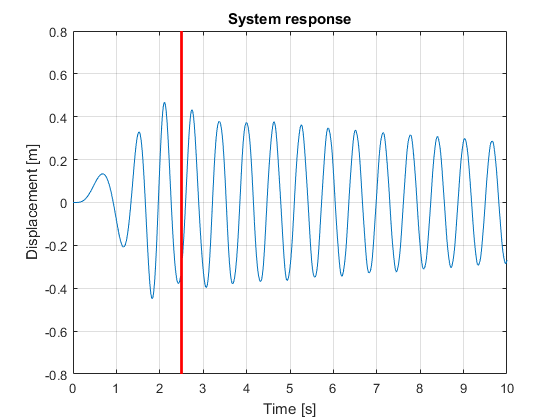
\includegraphics[width=\textwidth]{forced_response_fast.png}
			\caption{Response, $\omega = 4 t$ .}
		\end{subfigure}
		\caption{Forced response comparison. Solver ode45, default options. Vertical line designates damped natural frequency.}
		\label{fig:forced_response}
	\end{figure}
\end{document}